\documentclass{article}
\usepackage[dvipsnames]{xcolor}
\usepackage[final]{nips_2017}
\usepackage[utf8]{inputenc} % allow utf-8 input
\usepackage[T1]{fontenc}    % use 8-bit T1 fonts
\usepackage{hyperref}       % hyperlinks
\usepackage{url}            % simple URL typesetting
\usepackage{booktabs}       % professional-quality tables
\usepackage{amsfonts}       % blackboard math symbols
\usepackage{nicefrac}       % compact symbols for 1/2, etc.
\usepackage{microtype}      % microtypography
\usepackage{graphicx}
\usepackage{comment}
\usepackage{tikz}
\usetikzlibrary{tikzmark}
\usepackage{subcaption}
\usepackage{hanging}

\title{Stock Movement Prediction using Technical and  Data}

\author{
  Dylan M. Crain\\
  Stanford Department of Energy Resources Engineering\\
  736 Serra St., Stanford CA, 94305 \\
  \texttt{cooper96@stanford.edu} \\
  %% examples of more authors
  %% \And
  %% Coauthor \\
  %% Affiliation \\
  %% \texttt{email} \\
  %% \AND
  %% Coauthor \\
  %% Affiliation \\
  %% Address \\
  %% \texttt{email} \\
  %% \And
  %% Coauthor \\
  %% Affiliation \\
  %% Address \\
  %% \texttt{email} \\
  %% \And
  %% Coauthor \\
  %% Affiliation \\
  %% Address \\
  %% \texttt{email} \\
}

\begin{document}

\begin{center}
\includegraphics[width=3cm, height=0.7cm]{CS230}
\end{center}

\maketitle

\section{Abstract}

Stock price prediction is a notoriously challenging problem. Typically, when
trying to solve it, researchers and individuals use either technical 
(prices and volumes) or fundamental (text-based) data. However, it is exceedingly
rare for both forms to be used. This work utilizes Tesla data with sentiment analysis
performed on news titles pertaining to the company as well as technical data on its stock
over a three year period in order to predict closing price movement. For a next day
prediction, the final model architecture (a blended model) results in an
accuracy of 65\%, which is just under the highest accuracy observed in the
literature review. Also, as time to predict goes from 1 day to 3, the GRU model
does not have a large drop in accuracy, which insinuates it could be used for
later predictions.

\section{Introduction}

Stock price prediction is a classic and challenging problem at the intersection
of finance and computer science. Apart from the relatively heuristic behavior of
the market adding to these complications, there is a general sparsity of
data to work with for training a deep learning model. To be clear, there are
two primary types of data used in stock price prediction: technical and fundamental.

The former of these two data types, technical, refers to historic stock prices
and volumes (along with other such associated data). The latter of the two,
fundamental, applies to the type of data that investors look at on a
day-to-day basis to make their financial decisions. More often than not, this
information is text-based in the form of news articles and social media posts.

Due to technical data being easier, in general, to come by, most authors
solely use technical data to train deep learning models (Jiang [2021]).
These authors report varying success from this approach. An argument against the
strategy comes from Famma [1965] who claims an \textit{Efficient Market
Hypothesis (EMH)}, which states that all available information on the market is
tied up within technical data.

Due to this, some authors attempt to use fundamental (text-based) data to train
their deep learning prediction architectures instead (Hu et al. [2018]).
However, it is much rarer to see researchers mix the two approaches, i.e., to
combine both technical and fundamental data into the training of their models.

Thus, the goal of this work is to do just that: to combine both data streams in
the
prediction of stock movement in the future. This contribution, it is hoped, will help
add some validity to the proposed method and push the field forward towards more
accurate predictions. Secondly, most works only attempt to predict next of day
closing price. This work predicts stock price movement at more than one time
frame of 1 day, 3 days, and 5 days.

The input to this problem setup is a time-based sequence of
opening price, closing price, volume traded, high price, low price, and a
sentiment analysis metric applied to pertinent news articles for Tesla stock for ten days
leading up to the prediction. This work implements three architectures to use this
input to make predictions: LSTM, GRU, and a blended ensemble (BE)
which combines both of the previously mentioned base models.

\section{Related Work}

As mentioned previously, one approach for categorizing previous works on deep
learning assisted stock prediction is to determine whether the paper used
technical (Nabipour et al. [2020], Hiransha et al. [2018], and Kamalov et al.
[2021], and Stoean et al. [2018]), fundamental (Li \& Pan [2021] and Hu et al. [2018]), or (much more rarely) a combination of both data sources
When fundamental data is used, it can be interpreted in different ways.
Previously, there were many architectures that used an embedding,
usually coupled with a CNN architecture, to quantify the text-based information
(Vargas et al. [2017])

Currently, there has been a high interest paid to using sentiment
analysis on the text instead of embedding. This is useful since the goal
is to learn investor behavior. How a potential investor feels about
an article is generally more important to the problem at hand than how the
embedding relates to the movement of the stock.
Hu et al. [2018] used a highly complex and customized structure
to tease out sentiment as well as attention on given articles for input into
their overarching deep learning model. A more popular approach is to use a
pre-trained sentiment model to provide scores to text-based resources that are
associated with a given stock. Yang \& Yi [2021] uses one such model known as Valence Aware
Dictionary for Sentiment Reasoning (VADER), which is a lexicon based system trained
on social media posts. As this approach appears to be the current trend in the field,
VADER is used on the fundamental data in this work.

Continuing the trends of dealing with fundamental data, all of the works
reviewed used news articles as the fundamental information in their models.
Ding et al. [2014] advised that news titles
contained sufficient information to represent the articles.
Again, this is due
to trying to predict human response to a given article.
Moreover, Ding et al. claimed that utilizing the body of articles in training
a model may add unwanted noise.

The metrics used in the literature to measure how well the predictions are
performing, along with what is predicted, are quite varied.
Two popular forms of structuring the prediction are to either predict the price of
the stock at a given time or predict the movement of the stock, e.g., up or down,
. Predicting actual stock prices through regression, although
oftentimes resulting in astonishingly low mean squared errors, can be
misleading. If one looks closely at a comparison between the
predictions and true prices, the prediction
tends to predict based on the previous stock price. This is because stock
markets are highly heuristic. Thus, it is often concluded in more recent papers
that a much better prediction is stock relative movement (Jiang [2021]).
The appropriate metric to measure this prediction is the mean absolute
percentage error (MAPE) or ``accuracy'' in keras.

The final important insight from the literature review is the current standing
in model architecture for stock prediction. For this problem, many different
architectures have been utilized including: dense networks, CNNs, LSTM, GRU, 
and hybrid methods. Jiang [2021] displays that in the past few years the field has
been dominated by RNN model types, e.g., LSTM and GRU, as well as hybrid models.

In this work, the blended architecture from Li \& Pan [2021] is used along with the base
architectures of layered LSTM and GRU, since it was found to be especially
compelling by achieving the highest accuracy in the literature review at 67\%.

\section{Dataset \& Features}

All of the data used in this work is for Tesla. The technical data is composed
of the following five features: Closing Price, Volume, Open Price, High Price,
and Low Price for each trading day. This data was freely available by NASDAQ
for a ten year period from November 24, 2021.

Fundamental data was also gathered from NASDAQ, which 
gather its articles from sites such as: The Motley Fool, Reuters, and Trefis. 
The news articles in this set
go back to 2010. It is important to note, however, that although far reaching,
these news reports became increasingly sparse as time went on. It was determined
that three years, i.e., to November 24, 2018, was the practical limit before the
sparsity of news reports on trading days was too much to bear. Thus, the entire
data set had to be reduced from an initial length of ten years to three,
since the features through time must match. In fact, this is one of the
limitations of using fundamental data; it is harder to come by.

With news article titles over three years collected, VADER was applied to each news
title to determine whether the sentiment was positive or negative
towards Tesla. The VADER model predictions range from 1 to -1 with 1 signifying
an extremely positive sentiment and -1 being an extremely negative one. VADER
has been shown to have almost no difference with human decision making (Kirlic
\& Orhan [2017]), so it is used with confidence in this work.

\begin{table}
	\centering
	\caption{Tail of the data set (before sequencing) that includes the date of
	interest, technical data, and fundamental data scores.}
	\begin{tabular}{c c c c c c c}
		\toprule
		Date & Close & Volume & Open & High & Low & Scores\\
		\midrule
		11/18/21 & 1096.38 & 20898930 & 1106.55 & 1112 & 1075.02 & -0.0452\\
		11/19/21 & 1137.06 & 21642260 & 1098.87 & 1138.72 & 1092.70 & -0.1198\\
		11/22/21 & 1156.87 & 33072510 & 1162.33 & 1201.95 & 1132.43 & 0.1893\\
		11/23/21 & 1109.03 & 36171700 & 1167.51 & 1180.50 & 1062.70 & -0.0233\\
		11/24/21 & 1116 & 22560240 & 1080.39 & 1132.77 & 1062 & 0.1004\\
		\bottomrule
	\end{tabular}
	\label{tbl:dataset}
\end{table}

The sentiment scores are averaged over a given trading day with the assumption
that it is unlikely there will be a positive and negative association with Tesla
from the news reports in a single day. Furthermore, if there is no article
available for a given day, then the sentiment score is set to neutral (zero).
This is justified by the fact that if there was no report, then no sentiment can
be drawn from it anyway. A sample of the data set is displayed in
Table~\ref{tbl:dataset}.

As an example of the results from VADER, one of the higher scored titles had a
value of 0.8979 with text of ``Tesla shares surge 10\% as strong deliveries
drive profit optimism''. On the other hand, the lowest VADER sentiment score had
a value of -0.8934 with an associated article title of ``U.S. probing fatal
Tesla crash that killed pedestrian''. From these samples, it appears that the
VADER sentiment analysis is providing telling information on how
positive or negative news related to Tesla may be viewed.

All of the features were normalized between zero and one to prevent large
values, such as the volume feature, from having an unequal contribution to the
predictions. Furthermore, due to only having three years of useful data, the
number of dates of information are 746, since weekends and holidays do not
observe trading. This is a very small data set, but it is not unheard of. Li \&
Pan [2021]
had a data set half this size and Vargas et al. [2017] was also smaller. This sparsity of data is
one of the inherent problems of stock price prediction, especially when
fundamental data is included.

Finally, the data set is split into train/validate/test with 666/40/40
sequences, respectively. This means that the validation and test cases are around two months
of trading days each. Furthermore, the data set is split with temporal
consistency. That is, the training set is continuous from the latest day, the
validation set picks up from this to the test set, and it continues to the most
recent day of November 24, 2021. This is a common practice for these problems as
displayed in Kamalov et al. [2021].

\section{Methods}

\begin{figure}
	\begin{subfigure}[b]{0.45\textwidth}
		\centering
		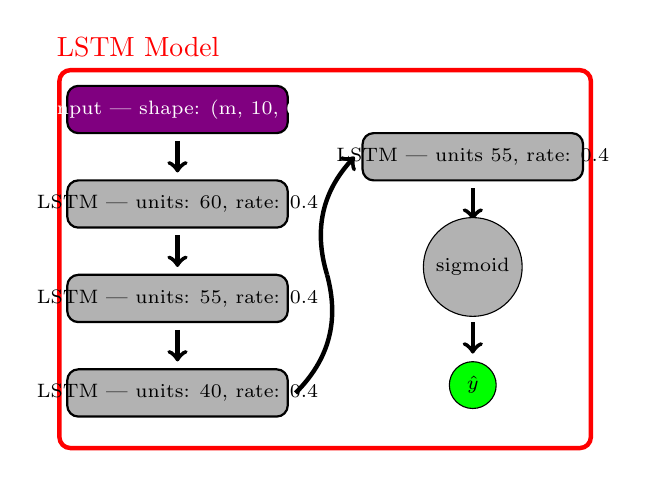
\begin{tikzpicture}
			\node at (1, 4.3) {\textcolor{red}{LSTM Model}};
			\draw [ultra thick, red, rounded corners] (0, -0.8) rectangle (6.75, 4);

			\draw [thick, black, rounded corners, fill=violet] (0.1, 3.8) rectangle
			(2.9, 3.2);
			\node [white] at (1.5, 3.5) {\scriptsize Input | shape: (m, 10, 6)};

			\draw [ultra thick, ->] (1.5, 3.1) -- (1.5, 2.7);

			\draw [thick, black, rounded corners, fill=black!30] (0.1, 2.6)
			rectangle (2.9, 2.0);
			\node [black] at (1.5, 2.3) {\scriptsize LSTM | units: 60, rate:
			0.4};

			\draw [ultra thick, ->] (1.5, 1.9) -- (1.5, 1.5);

			\draw [thick, black, rounded corners, fill=black!30] (0.1, 1.4)
			rectangle (2.9, 0.8);
			\node [black] at (1.5, 1.1) {\scriptsize LSTM | units: 55, rate:
			0.4};

			\draw [ultra thick, ->] (1.5, 0.7) -- (1.5, 0.3);

			\draw [thick, black, rounded corners, fill=black!30] (0.1, 0.2)
			rectangle (2.9, -0.4);
			\node [black] at (1.5, -0.1) {\scriptsize LSTM | units: 40, rate:
			0.4};

			\draw [ultra thick] (3.0, -0.1) to[bend right] (3.4, 1.4);
			\draw [ultra thick, ->] (3.4, 1.4) to[bend left] (3.75, 2.9);

			\draw [thick, black, rounded corners, fill=black!30] (3.85, 3.2)
			rectangle (6.65, 2.6);
			\node [black] at (5.25, 2.9) {\scriptsize LSTM | units 55, rate: 0.4};

			\draw [ultra thick, ->] (5.25, 2.5) -- (5.25, 2.1);

			\node [circle, draw, fill=black!30] (c) at (5.25, 1.5) {\scriptsize sigmoid};
			
			\draw [ultra thick, ->] (5.25, 0.8) -- (5.25, 0.4);

			\node [circle, draw, fill=green] (c) at (5.25, 0.0) {\scriptsize $\hat{y}$};
		\end{tikzpicture}
		\label{fig:lstm}
	\end{subfigure}
	\hfill
	\begin{subfigure}[b]{0.45\textwidth}
		\centering
		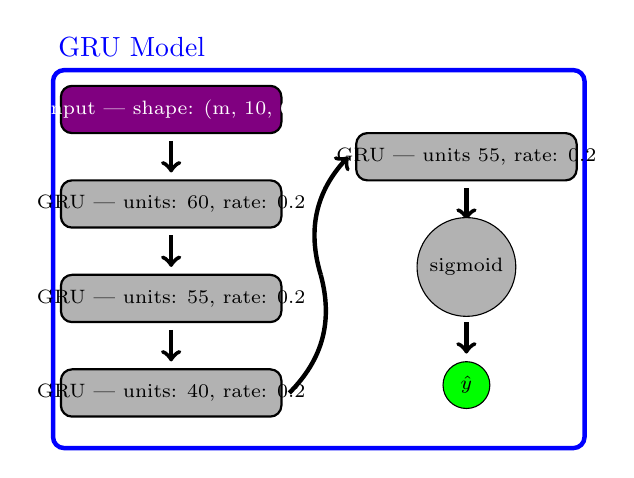
\begin{tikzpicture}
			\node at (1, 4.3) {\textcolor{blue}{GRU Model}};
			\draw [ultra thick, blue, rounded corners] (0, -0.8) rectangle (6.75, 4);

			\draw [thick, black, rounded corners, fill=violet] (0.1, 3.8) rectangle
			(2.9, 3.2);
			\node [white] at (1.5, 3.5) {\scriptsize Input | shape: (m, 10, 6)};

			\draw [ultra thick, ->] (1.5, 3.1) -- (1.5, 2.7);

			\draw [thick, black, rounded corners, fill=black!30] (0.1, 2.6)
			rectangle (2.9, 2.0);
			\node [black] at (1.5, 2.3) {\scriptsize GRU | units: 60, rate:
			0.2};

			\draw [ultra thick, ->] (1.5, 1.9) -- (1.5, 1.5);

			\draw [thick, black, rounded corners, fill=black!30] (0.1, 1.4)
			rectangle (2.9, 0.8);
			\node [black] at (1.5, 1.1) {\scriptsize GRU | units: 55, rate:
			0.2};

			\draw [ultra thick, ->] (1.5, 0.7) -- (1.5, 0.3);

			\draw [thick, black, rounded corners, fill=black!30] (0.1, 0.2)
			rectangle (2.9, -0.4);
			\node [black] at (1.5, -0.1) {\scriptsize GRU | units: 40, rate:
			0.2};

			\draw [ultra thick] (3.0, -0.1) to[bend right] (3.4, 1.4);
			\draw [ultra thick, ->] (3.4, 1.4) to[bend left] (3.75, 2.9);

			\draw [thick, black, rounded corners, fill=black!30] (3.85, 3.2)
			rectangle (6.65, 2.6);
			\node [black] at (5.25, 2.9) {\scriptsize GRU | units 55, rate: 0.2};

			\draw [ultra thick, ->] (5.25, 2.5) -- (5.25, 2.1);

			\node [circle, draw, fill=black!30] (c) at (5.25, 1.5) {\scriptsize sigmoid};
			
			\draw [ultra thick, ->] (5.25, 0.8) -- (5.25, 0.4);

			\node [circle, draw, fill=green] (c) at (5.25, 0.0) {\scriptsize $\hat{y}$};
		\end{tikzpicture}
		\label{fig:gru}
	\end{subfigure}
	\caption{Architecture of base models. Note that the input shape is batch
	size, time step, and feature size respectively.}
	\label{fig:base}
\end{figure}

\begin{figure}
	\centering
	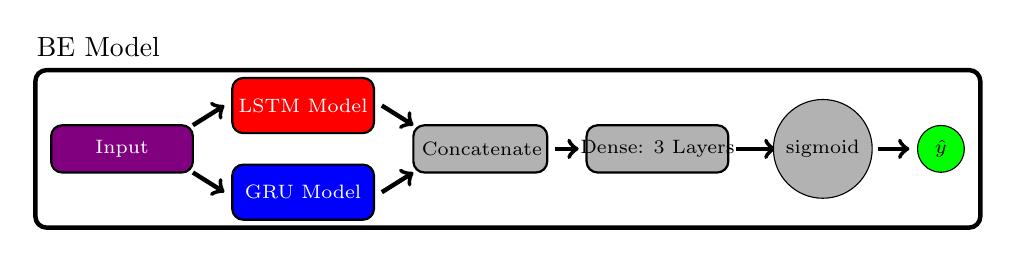
\begin{tikzpicture}
		\node at (0.8, 2.3) {BE Model};
		\draw [ultra thick, black, rounded corners] (0, 0) rectangle (12, 2);

		 \draw [thick, black, rounded corners, fill=violet] (0.2, 0.7)
		 rectangle (2, 1.3);
		 \node [white] at (1.1, 1.0) {\scriptsize Input};

		 \draw [ultra thick, ->] (2, 1.3) -- (2.4, 1.55);
		 \draw [ultra thick, ->] (2, 0.7) -- (2.4, 0.45);

		 \draw [thick, black, rounded corners, fill=red] (2.5, 1.2) rectangle
		 (4.3, 1.9);
		 \node [white] at (3.4, 1.55) {\scriptsize LSTM Model};

		 \draw [ultra thick, ->] (4.4, 1.55) -- (4.8, 1.3);

		 \draw [thick, black, rounded corners, fill=blue] (2.5, 0.8) rectangle
		 (4.3, 0.1);
		 \node [white] at (3.4, 0.45) {\scriptsize GRU Model};

		 \draw [ultra thick, ->] (4.4, 0.45) -- (4.8, 0.7);

		 \draw [thick, black, rounded corners, fill=black!30] (4.8, 0.7)
		 rectangle (6.5, 1.3);
		 \node at (5.67, 1.0) {\scriptsize Concatenate};
		 
		 \draw [ultra thick, ->] (6.6, 1.0) -- (6.9, 1.0);

		 \draw [thick, black, rounded corners, fill=black!30] (7.0, 0.7)
		 rectangle (8.8, 1.3);
		 \node at (7.9, 1.0) {\scriptsize Dense: 3 Layers};

		 \draw [ultra thick, ->] (8.9, 1.0) -- (9.4, 1.0);

		 \node [circle, draw, fill=black!30] (c) at (10, 1.0) {\scriptsize
		 sigmoid};

		 \draw [ultra thick, ->] (10.7, 1.0) -- (11.1, 1.0);

		 \node [circle, draw, fill=green] (c) at (11.5, 1.0) {\scriptsize
		 $\hat{y}$};

	\end{tikzpicture}
	\caption{Architecture of the blended ensemble model that uses the trained
	LSTM and GRU models to arrive at its predictions.}
	\label{fig:big}
\end{figure}

The first step of all methods used is to convert the raw data from
Table~\ref{tbl:dataset} into a time sequence representation and normalize the
features. Deciding on the horizon, or the number of days prior to prediction to
include information, is crucial to stock prediction. 
If too short a window is chosen, then only compulsive
reactions are captured; whereas if too large a window is used, then the data
used has likely escaped an investor's memory. Over many iterations, \textbf{ten
days} was used as the number of days prior to predictions.

In terms of other hyperparameters, many were iterated over. This was mainly done
to prevent overfitting, which was quite a problem to overcome due to the small
data set size. The hyperparameters scaled include: layers, units in layer, dropout
rate, optimizer, learning rate, batch size, and epoch size.

Three different architectures were utilized on this data set. The first (seen in
Figure~\ref{base} is an
LSTM model with four layers. The number of units in each layer are 60, 55, 50,
and 45, respectively with each layer experiencing a dropout rate of 0.4. The
number of epochs used was 150. For this
model, as well as for the GRU model, the batch size was 16; learning rate was
slightly less than the default at 0.0008, and the best optimizer was determined
to be RMSprop. Finally, the results are input into a single node with sigmoid
activation to predict the direction of the stock -- 1 for up, and 0 for down.

The second model was a layered GRU (Figure~\ref{fig:base}) with the same number
of layers and units in
each layer as the LSTM model. The dropout for the GRU, however, was less severe
with a rate of 0.2 for each layer. Furthermore, the number of epochs used was
slightly larger at 200. Note that a batch size of 16 was chosen due to the small
number of training examples.

The final model used on the data set is a blended ensemble that is
described in Li \& Pan [2021]. Essentially, the two fully trained LSTM and GRU models are
combined to improve the prediction. After training the base models on the training set,
each model is used to predict the validation results.
These predictions are combined into a new data set of dimensions $p
\times 2$, where $p$ is the number of predictions, one for each sequence, and 2
is for the two models used for prediction.

This new data set is fed into a dense, three layered model to predict the
validation set, i.e., the validation predictions from the base models train the
BE model.  Note that the dense portion has
three hidden layers with the following node counts: 30, 25, and 20 with a Relu
activation in each node. As before, the final result is sent to a single node
with a sigmoid activation. The optimizer used here is Adam with 100 epochs, and
a batch size of 8 is used due to the validation set being much smaller than
the training set.

Finally, with the BE trained, the predictions of GRU and LSTM are found on the
test set and ran through the dense layers to get the test prediction. Note that
since the prediction is binary (1 for upward movement and 0 for downward), the
binary cross-entropy loss function is used for all of the models discussed.

\section{Results \& Discussion}

\begin{table}
	\centering
	\caption{Results over the three models with predicting 1, 3, or 5 days
	ahead. Of those trained, the maximum accuracies are \textbf{bold}.}
	\begin{tabular}{c c c c}
		\toprule
		Model & Day 1 Prediction & Day 3 Prediction & Day 5 Prediction\\
		\midrule
		LSTM & 36.25\% & 22.12\% & 17.85\%\\
		GRU & 59.35\% & \textbf{52.67}\% & \textbf{26.75}\%\\
		BE & \textbf{65.12}\% & -- & -- \\
		\bottomrule
	\end{tabular}
	\label{tbl:results}
\end{table}

The final accuracy results for each setup is shown in Table~\ref{tbl:results}.
For the LSTM and GRU models, movement predictions were made for 1, 3, and 5 days
into the future, with only the 1 day prediction considered for the BE model due
to time constraints.

The LSTM model was the first trained and used for prediction on the test set
with one day into the future.  The accuracy, as displayed, is low at only
36.25\%. One expects a random guess to result in an accuracy of 50\%,
so this result seems suspect. However, it is not unheard of.
In Li \& Pan [2021] and Nabipour et al. [2020] the LSTM models used to predict movement a day into the future
have accuracies of 33.33\% and 43\% respectively.

Due to concern on the accuracy of the LSTM model, a GRU was used well, since
Li \& Pan [2021] mentioned that it could be more accurate when little data is available. This
proved true with the GRU model having a prediction accuracy of 59.35\% for a one
 day prediction.

Adusumilli [2019] noted that if a predicting model could achieve 60\% accuracy or more, then
major profits can be made. In an attempt to reach this goal, the blended
ensemble (BE) was utilized. The accuracy for a next of day prediction was
65.12\%. This value is just shy of the largest accuracy found in the
literature review at 67\% Li \& Pan [2021].

For the longer prediction periods of 3 and 5 days, the accuracy predictably went
down. However, for the GRU the decrease from a next of day prediction to 3 days
is much lower (7 percentage points) then was expected. This means that there may
be hope in accurate stock predictions beyond the next day movement.

\section{Conclusions \& Future Work}

In order to move the challenging field of stock prediction forward, this work
explores the capability of using a sentiment analysis to include fundamental as
well as technical data into training a deep learning model in the prediction of
stock movement. A single stock (Tesla) is utilized. Three
different models are showcased with the most complicated, blended ensemble,
achieving an accuracy of 65\%, which is the second largest accuracy found in the
extensive literature review performed. 
This high performance points to the utility and returns
possible from utilizing both fundamental and technical data in stock prediction.

During this work, it was found that the attainment of fundamental
(textual) data such as pertinent news report titles was a limiting factor. The
availability of such information was dubious at best and even then it became
incredibly sparse as time went on. With the utility of using fundamental data
supported by this work, the availability of an open source data base of stock
pertinent news articles and social media posts could be indispensable.

Furthermore, if more time were available, it would be a useful alteration to
include more than just one stock in the analysis. This would make prediction
more challenging, but, at the same time, there are likely to be correlations
between different companies that may be learned by the model architecture.

Moreover, weighting of the features could be an interesting direction to take.
In this work, each feature (5 of which were technical) was weighted equally with
only one being associated with fundamental data. This likely reduced the effect
of the textual information on the training of the model. Increasing the weight
of this feature could prove to be another hyperparameter or other text-based
features could be included to give more weight to this type of information.

\section{References}

\begin{hangparas}{0.25in}{1}
Adusumilli, R.:PredictingstockpricesusingakerasLSTMmodel. NikolaNews (2019)

Akita, R., Yoshihara, A., Matsubara, T., \& Uehara, K. (2016, June). Deep learning for stock prediction using numerical and textual information. In 2016 IEEE/ACIS 15th International Conference on Computer and Information Science (ICIS) (pp. 1-6). IEEE.

Chollet, F., \& others. (2015). Keras. GitHub. Retrieved from https://github.com/fchollet/keras

Ding, X., Zhang, Y., Liu, T., Duan, J.: Using structured events to predict stock price movement: an empirical investigation. In: Proceedings of the 2014 Conference on Empirical Methods in Nat- ural Language Processing (EMNLP), pp. 1415–1425. Association for Computational Linguistics (2014). https://doi.org/10.3115/v1/ D14-1148

Fama, E. F. (1965). The behavior of stock-market prices. The Journal of Business, 38, 34-105.

Harris, C.R., Millman, K.J., van der Walt, S.J. et al. Array programming with NumPy. Nature 585, 357–362 (2020). DOI: 10.1038/s41586-020-2649-2. 

Hiransha, M., Gopalakrishnan, E. A., Menon, V. K., \& Soman, K. P. (2018). NSE stock market prediction using deep-learning models. Procedia computer science, 132, 1351-1362.

Hu, Z., Liu, W., Bian, J., Liu, X., Liu, T.: Listening to chaotic whispers: a deep learning framework for news-oriented stock trend prediction. In: Proceedings of the Eleventh ACM International Conference on Web Search and Data Mining, WSDM (2018). https://doi.org/10.1145/3159652.3159690

Jiang, W. (2021). Applications of deep learning in stock market prediction:

Kamalov, F., Smail, L., \& Gurrib, I. (2020, November). Stock price forecast with deep learning. In 2020 International Conference on Decision Aid Sciences and Application (DASA) (pp. 1098-1102). IEEE.

Kirlic ́, A., Orhan, Z.: Measuring human and Vader performance on sentiment analysis. Invent. J. Res. Technol. Eng. Manag. (IJRTEM) 1, 42–46 (2017)

Li, Y., \& Pan, Y. (2021). A novel ensemble deep learning model for stock prediction based on stock prices and news. International Journal of Data Science and Analytics, 1-11.

Martín Abadi, Ashish Agarwal, Paul Barham, Eugene Brevdo,
Zhifeng Chen, Craig Citro, Greg S. Corrado, Andy Davis,
Jeffrey Dean, Matthieu Devin, Sanjay Ghemawat, Ian Goodfellow,
Andrew Harp, Geoffrey Irving, Michael Isard, Rafal Jozefowicz, Yangqing Jia,
Lukasz Kaiser, Manjunath Kudlur, Josh Levenberg, Dan Mané, Mike Schuster,
Rajat Monga, Sherry Moore, Derek Murray, Chris Olah, Jonathon Shlens,
Benoit Steiner, Ilya Sutskever, Kunal Talwar, Paul Tucker,
Vincent Vanhoucke, Vijay Vasudevan, Fernanda Viégas,
Oriol Vinyals, Pete Warden, Martin Wattenberg, Martin Wicke,
Yuan Yu, and Xiaoqiang Zheng.
TensorFlow: Large-scale machine learning on heterogeneous systems,
2015. Software available from tensorflow.org.

Nabipour, M., Nayyeri, P., Jabani, H., Mosavi, A., \& Salwana, E. (2020). Deep learning for stock market prediction. Entropy, 22(8), 840.

Pedregosa, F., Varoquaux, Ga"el, Gramfort, A., Michel, V., Thirion, B., Grisel, O., … others. (2011). Scikit-learn: Machine learning in Python. Journal of Machine Learning Research, 12(Oct), 2825–2830.

Vargas, M. R., De Lima, B. S., \& Evsukoff, A. G. (2017, June). Deep learning for stock market prediction from financial news articles. In 2017 IEEE international conference on computational intelligence and virtual environments for measurement systems and applications (CIVEMSA) (pp. 60-65). IEEE.

Daily stock market overview, data updates, reports \&amp; news. Nasdaq. (n.d.). Retrieved December 3, 2021, from https://www.nasdaq.com/.
\end{hangparas}

\end{document}
